\documentclass[../../main.tex]{subfiles}
\begin{document}

{\bf [解]}

\begin{figure}[htb]
  \centering
  \begin{tikzpicture}[x=1.5cm, y=1.0cm, >=stealth, every node/.style={font=\small}]
    % 数直線
    \draw[->, thick, gray!80!black] (-0.5, 0) -- (5.8, 0) node[right] {$x$};
    \draw[thick, gray!80!black] (0, 0.08) -- (0, -0.08) node[below=2pt] {$0$};
    \draw[dashed, gray!60] (1.8, 2.0) -- (1.8, 0) node[below=2pt, gray!80!black] {$2$};
    \draw[dashed, gray!60] (3.4, 1.0) -- (3.4, 0) node[below=2pt, blue!85!black] {$f(t)$};
    \draw[dashed, gray!60] (4.6, 1.0) -- (4.6, 0) node[below=2pt, teal!85!black] {$g(t)$};

    % t = 0
    \node[left=6pt, font=\footnotesize] at (-0.2, 2.0) {時刻 $t = 0$：};
    \node[circle, fill=blue!85!black, inner sep=1.3pt] at (0, 2.0) {};
    \node[above=2pt, font=\footnotesize, blue!85!black] at (0, 2.0) {$A$};
    \draw[->, thick, blue!85!black] (0.2, 2.0) -- (1.25, 2.0) node[midway, above=1pt, font=\scriptsize] {$u=t^2+5$};
    \node[circle, fill=teal!85!black, inner sep=1.3pt] at (1.8, 2.0) {};
    \node[above=2pt, font=\footnotesize, teal!85!black] at (1.8, 2.0) {$B$};
    \draw[->, thick, teal!85!black] (2.0, 2.0) -- (2.8, 2.0) node[midway, above=1pt, font=\scriptsize] {$v=5t$};

    % 一般の時刻 t
    \node[left=6pt, font=\footnotesize] at (-0.2, 1.0) {時刻 $t$：};
    \node[circle, fill=blue!85!black, inner sep=1.3pt] at (3.4, 1.0) {};
    \node[above=2pt, font=\footnotesize, blue!85!black] at (3.4, 1.0) {$A$};
    \node[circle, fill=teal!85!black, inner sep=1.3pt] at (4.6, 1.0) {};
    \node[above=2pt, font=\footnotesize, teal!85!black] at (4.6, 1.0) {$B$};
  \end{tikzpicture}
  \caption{数直線上における A と B の出発位置と時刻 $t$ での位置}
  \label{fig:1961_6_number_line}
\end{figure}

A の出発点を $0$ とする．時刻 $t$ での A, B の位置 $f(t), g(t)$ とすると題意から
\begin{align}
  \begin{cases}
    f(t) = \int_0^t (p^2 + 5) dp = \dfrac{1}{3} t^3 + 5t \\
    g(t) = 2 + \int_0^t 5p dp = \dfrac{5}{2} t^2 + 2
  \end{cases}
\end{align}
だから $0 \le t \le 4$ で $f(t) = g(t)$ となる $t$ の数を求めればよい．
$h(t) = f(t) - g(t)$ とおくと，これは $h(t) = 0$ となる $t$ の数にひとしい．
一階微分を計算すると
\begin{align}
  h'(t) &= t^2 + 5 - 5t \\
  &= \left(t - \dfrac{5-\sqrt{5}}{2}\right)\left(t - \dfrac{5+\sqrt{5}}{2}\right)
\end{align}
から増減表と$h(t)$のグラフの概形は以下のようになる．

\begin{table}[htb]
  \centering
  \caption{$h(t)$ の増減表（$0 \le t \le 4$）}
  \label{tab:1961_6_ht_variation}
  \renewcommand{\arraystretch}{1.5}
  \begin{tabular}{c|cccccc|c}
    \hline
    $t$ & $0$ & $\dots$ & $\dfrac{5-\sqrt{5}}{2}$ & $\dots$ & $\dfrac{5+\sqrt{5}}{2}$ & $\dots$ & $4$ \\ \hline
    $h'$ & & $+$ & $0$ & $-$ & $0$ & $+$ & \\ \hline
    $h$ & $-2$ & $\nearrow$ & $\dfrac{1}{12}(1 + 5\sqrt{5})$ & $\searrow$ & $\dfrac{1}{12}(1 - 5\sqrt{5})$ & $\nearrow$ & $-\dfrac{2}{3}$ \\ \hline
  \end{tabular}
\end{table}

\begin{figure}[htb]
  \centering
  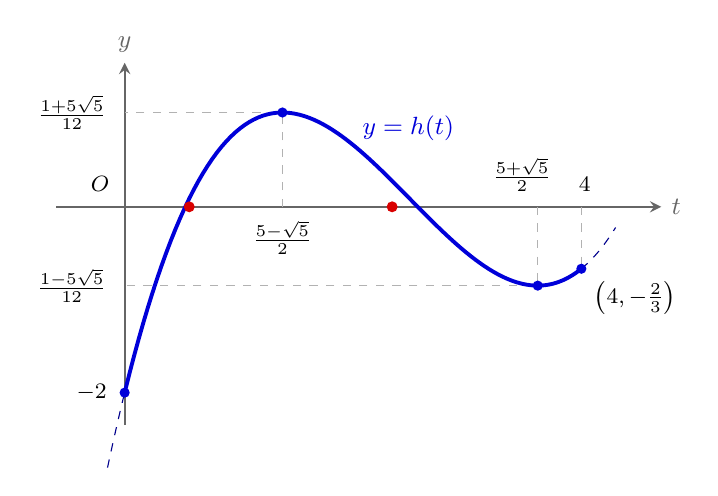
\begin{tikzpicture}[x=1.45cm, y=1.18cm, >=stealth, every node/.style={font=\small}]
    % 極値を与える t1=(5-sqrt(5))/2 ≈ 1.3820, t2=(5+sqrt(5))/2 ≈ 3.6180
    % h(t1) = (1+5*sqrt(5))/12 ≈ 1.0150, h(t2) = (1-5*sqrt(5))/12 ≈ -0.8484
    \coordinate (O)  at (0, 0);
    \coordinate (P0) at (0, -2.0);
    \coordinate (P1) at (1.3820, 1.0150);
    \coordinate (P2) at (3.6180, -0.8484);
    \coordinate (P4) at (4.0, -0.6667);
    \coordinate (R1) at (0.5657, 0);
    \coordinate (R2) at (2.3429, 0);

    % 座標軸
    \draw[->, thick, gray!80!black] (-0.6, 0) -- (4.7, 0) node[right] {$t$};
    \draw[->, thick, gray!80!black] (0, -2.35) -- (0, 1.55) node[above] {$y$};
    \node[above left=2pt, font=\footnotesize] at (O) {$O$};

    % 投影線（破線）
    \draw[dashed, gray!60] (1.3820, 0) -- (P1) -- (0, 1.0150);
    \draw[dashed, gray!60] (3.6180, 0) -- (P2) -- (0, -0.8484);
    \draw[dashed, gray!60] (4.0, 0) -- (P4);

    % 定義域外の延長（破線）と [0, 4] 上の曲線 y = h(t)
    \draw[dashed, blue!55!black, domain=-0.15:0, samples=15]
    plot (\x, {(\x)^3/3 - 2.5*(\x)^2 + 5*(\x) - 2});
    \draw[dashed, blue!55!black, domain=4.0:4.3, samples=20]
    plot (\x, {(\x)^3/3 - 2.5*(\x)^2 + 5*(\x) - 2});
    \draw[line width=1.4pt, blue!85!black, domain=0:4, samples=100]
    plot (\x, {(\x)^3/3 - 2.5*(\x)^2 + 5*(\x) - 2});
    \node[above right=2pt, blue!85!black] at (1.95, 0.55) {$y=h(t)$};

    % 点とラベル
    \node[circle, fill=blue!85!black, inner sep=1.3pt] at (P0) {};
    \node[left=3pt, font=\footnotesize] at (P0) {$-2$};

    \node[circle, fill=blue!85!black, inner sep=1.3pt] at (P1) {};
    \node[below=2pt, font=\footnotesize, fill=white, inner sep=1.5pt] at (1.3820, -0.04) {$\frac{5-\sqrt{5}}{2}$};
    \node[left=3pt, font=\footnotesize] at (0, 1.0150) {$\frac{1+5\sqrt{5}}{12}$};

    \node[circle, fill=blue!85!black, inner sep=1.3pt] at (P2) {};
    \node[above=2pt, font=\footnotesize] at (3.48, 0) {$\frac{5+\sqrt{5}}{2}$};
    \node[left=3pt, font=\footnotesize] at (0, -0.8484) {$\frac{1-5\sqrt{5}}{12}$};

    \node[circle, fill=blue!85!black, inner sep=1.3pt] at (P4) {};
    \node[above=2pt, font=\footnotesize] at (4.03, 0) {$4$};
    \node[below right=1pt, font=\footnotesize] at (P4) {$\left(4, -\frac{2}{3}\right)$};

    % t 軸との交点（求める実数解 2 個）
    \node[circle, fill=red!85!black, inner sep=1.4pt] at (R1) {};
    \node[circle, fill=red!85!black, inner sep=1.4pt] at (R2) {};
  \end{tikzpicture}
  \caption{$y=h(t)$ のグラフ（$0 \le t \le 4$）}
  \label{fig:1961_6_ht_graph}
\end{figure}

よってグラフから求める$t$の数は$2$個である．

\end{document}
